% Options for packages loaded elsewhere
\PassOptionsToPackage{unicode}{hyperref}
\PassOptionsToPackage{hyphens}{url}
\PassOptionsToPackage{dvipsnames,svgnames,x11names}{xcolor}
%
\documentclass[
  letterpaper,
  DIV=11,
  numbers=noendperiod]{scrartcl}

\usepackage{amsmath,amssymb}
\usepackage{iftex}
\ifPDFTeX
  \usepackage[T1]{fontenc}
  \usepackage[utf8]{inputenc}
  \usepackage{textcomp} % provide euro and other symbols
\else % if luatex or xetex
  \usepackage{unicode-math}
  \defaultfontfeatures{Scale=MatchLowercase}
  \defaultfontfeatures[\rmfamily]{Ligatures=TeX,Scale=1}
\fi
\usepackage{lmodern}
\ifPDFTeX\else  
    % xetex/luatex font selection
\fi
% Use upquote if available, for straight quotes in verbatim environments
\IfFileExists{upquote.sty}{\usepackage{upquote}}{}
\IfFileExists{microtype.sty}{% use microtype if available
  \usepackage[]{microtype}
  \UseMicrotypeSet[protrusion]{basicmath} % disable protrusion for tt fonts
}{}
\makeatletter
\@ifundefined{KOMAClassName}{% if non-KOMA class
  \IfFileExists{parskip.sty}{%
    \usepackage{parskip}
  }{% else
    \setlength{\parindent}{0pt}
    \setlength{\parskip}{6pt plus 2pt minus 1pt}}
}{% if KOMA class
  \KOMAoptions{parskip=half}}
\makeatother
\usepackage{xcolor}
\setlength{\emergencystretch}{3em} % prevent overfull lines
\setcounter{secnumdepth}{-\maxdimen} % remove section numbering
% Make \paragraph and \subparagraph free-standing
\makeatletter
\ifx\paragraph\undefined\else
  \let\oldparagraph\paragraph
  \renewcommand{\paragraph}{
    \@ifstar
      \xxxParagraphStar
      \xxxParagraphNoStar
  }
  \newcommand{\xxxParagraphStar}[1]{\oldparagraph*{#1}\mbox{}}
  \newcommand{\xxxParagraphNoStar}[1]{\oldparagraph{#1}\mbox{}}
\fi
\ifx\subparagraph\undefined\else
  \let\oldsubparagraph\subparagraph
  \renewcommand{\subparagraph}{
    \@ifstar
      \xxxSubParagraphStar
      \xxxSubParagraphNoStar
  }
  \newcommand{\xxxSubParagraphStar}[1]{\oldsubparagraph*{#1}\mbox{}}
  \newcommand{\xxxSubParagraphNoStar}[1]{\oldsubparagraph{#1}\mbox{}}
\fi
\makeatother

\usepackage{color}
\usepackage{fancyvrb}
\newcommand{\VerbBar}{|}
\newcommand{\VERB}{\Verb[commandchars=\\\{\}]}
\DefineVerbatimEnvironment{Highlighting}{Verbatim}{commandchars=\\\{\}}
% Add ',fontsize=\small' for more characters per line
\usepackage{framed}
\definecolor{shadecolor}{RGB}{241,243,245}
\newenvironment{Shaded}{\begin{snugshade}}{\end{snugshade}}
\newcommand{\AlertTok}[1]{\textcolor[rgb]{0.68,0.00,0.00}{#1}}
\newcommand{\AnnotationTok}[1]{\textcolor[rgb]{0.37,0.37,0.37}{#1}}
\newcommand{\AttributeTok}[1]{\textcolor[rgb]{0.40,0.45,0.13}{#1}}
\newcommand{\BaseNTok}[1]{\textcolor[rgb]{0.68,0.00,0.00}{#1}}
\newcommand{\BuiltInTok}[1]{\textcolor[rgb]{0.00,0.23,0.31}{#1}}
\newcommand{\CharTok}[1]{\textcolor[rgb]{0.13,0.47,0.30}{#1}}
\newcommand{\CommentTok}[1]{\textcolor[rgb]{0.37,0.37,0.37}{#1}}
\newcommand{\CommentVarTok}[1]{\textcolor[rgb]{0.37,0.37,0.37}{\textit{#1}}}
\newcommand{\ConstantTok}[1]{\textcolor[rgb]{0.56,0.35,0.01}{#1}}
\newcommand{\ControlFlowTok}[1]{\textcolor[rgb]{0.00,0.23,0.31}{\textbf{#1}}}
\newcommand{\DataTypeTok}[1]{\textcolor[rgb]{0.68,0.00,0.00}{#1}}
\newcommand{\DecValTok}[1]{\textcolor[rgb]{0.68,0.00,0.00}{#1}}
\newcommand{\DocumentationTok}[1]{\textcolor[rgb]{0.37,0.37,0.37}{\textit{#1}}}
\newcommand{\ErrorTok}[1]{\textcolor[rgb]{0.68,0.00,0.00}{#1}}
\newcommand{\ExtensionTok}[1]{\textcolor[rgb]{0.00,0.23,0.31}{#1}}
\newcommand{\FloatTok}[1]{\textcolor[rgb]{0.68,0.00,0.00}{#1}}
\newcommand{\FunctionTok}[1]{\textcolor[rgb]{0.28,0.35,0.67}{#1}}
\newcommand{\ImportTok}[1]{\textcolor[rgb]{0.00,0.46,0.62}{#1}}
\newcommand{\InformationTok}[1]{\textcolor[rgb]{0.37,0.37,0.37}{#1}}
\newcommand{\KeywordTok}[1]{\textcolor[rgb]{0.00,0.23,0.31}{\textbf{#1}}}
\newcommand{\NormalTok}[1]{\textcolor[rgb]{0.00,0.23,0.31}{#1}}
\newcommand{\OperatorTok}[1]{\textcolor[rgb]{0.37,0.37,0.37}{#1}}
\newcommand{\OtherTok}[1]{\textcolor[rgb]{0.00,0.23,0.31}{#1}}
\newcommand{\PreprocessorTok}[1]{\textcolor[rgb]{0.68,0.00,0.00}{#1}}
\newcommand{\RegionMarkerTok}[1]{\textcolor[rgb]{0.00,0.23,0.31}{#1}}
\newcommand{\SpecialCharTok}[1]{\textcolor[rgb]{0.37,0.37,0.37}{#1}}
\newcommand{\SpecialStringTok}[1]{\textcolor[rgb]{0.13,0.47,0.30}{#1}}
\newcommand{\StringTok}[1]{\textcolor[rgb]{0.13,0.47,0.30}{#1}}
\newcommand{\VariableTok}[1]{\textcolor[rgb]{0.07,0.07,0.07}{#1}}
\newcommand{\VerbatimStringTok}[1]{\textcolor[rgb]{0.13,0.47,0.30}{#1}}
\newcommand{\WarningTok}[1]{\textcolor[rgb]{0.37,0.37,0.37}{\textit{#1}}}

\providecommand{\tightlist}{%
  \setlength{\itemsep}{0pt}\setlength{\parskip}{0pt}}\usepackage{longtable,booktabs,array}
\usepackage{calc} % for calculating minipage widths
% Correct order of tables after \paragraph or \subparagraph
\usepackage{etoolbox}
\makeatletter
\patchcmd\longtable{\par}{\if@noskipsec\mbox{}\fi\par}{}{}
\makeatother
% Allow footnotes in longtable head/foot
\IfFileExists{footnotehyper.sty}{\usepackage{footnotehyper}}{\usepackage{footnote}}
\makesavenoteenv{longtable}
\usepackage{graphicx}
\makeatletter
\def\maxwidth{\ifdim\Gin@nat@width>\linewidth\linewidth\else\Gin@nat@width\fi}
\def\maxheight{\ifdim\Gin@nat@height>\textheight\textheight\else\Gin@nat@height\fi}
\makeatother
% Scale images if necessary, so that they will not overflow the page
% margins by default, and it is still possible to overwrite the defaults
% using explicit options in \includegraphics[width, height, ...]{}
\setkeys{Gin}{width=\maxwidth,height=\maxheight,keepaspectratio}
% Set default figure placement to htbp
\makeatletter
\def\fps@figure{htbp}
\makeatother
% definitions for citeproc citations
\NewDocumentCommand\citeproctext{}{}
\NewDocumentCommand\citeproc{mm}{%
  \begingroup\def\citeproctext{#2}\cite{#1}\endgroup}
\makeatletter
 % allow citations to break across lines
 \let\@cite@ofmt\@firstofone
 % avoid brackets around text for \cite:
 \def\@biblabel#1{}
 \def\@cite#1#2{{#1\if@tempswa , #2\fi}}
\makeatother
\newlength{\cslhangindent}
\setlength{\cslhangindent}{1.5em}
\newlength{\csllabelwidth}
\setlength{\csllabelwidth}{3em}
\newenvironment{CSLReferences}[2] % #1 hanging-indent, #2 entry-spacing
 {\begin{list}{}{%
  \setlength{\itemindent}{0pt}
  \setlength{\leftmargin}{0pt}
  \setlength{\parsep}{0pt}
  % turn on hanging indent if param 1 is 1
  \ifodd #1
   \setlength{\leftmargin}{\cslhangindent}
   \setlength{\itemindent}{-1\cslhangindent}
  \fi
  % set entry spacing
  \setlength{\itemsep}{#2\baselineskip}}}
 {\end{list}}
\usepackage{calc}
\newcommand{\CSLBlock}[1]{\hfill\break\parbox[t]{\linewidth}{\strut\ignorespaces#1\strut}}
\newcommand{\CSLLeftMargin}[1]{\parbox[t]{\csllabelwidth}{\strut#1\strut}}
\newcommand{\CSLRightInline}[1]{\parbox[t]{\linewidth - \csllabelwidth}{\strut#1\strut}}
\newcommand{\CSLIndent}[1]{\hspace{\cslhangindent}#1}

\usepackage{booktabs}
\usepackage{caption}
\usepackage{longtable}
\usepackage{colortbl}
\usepackage{array}
\usepackage{anyfontsize}
\usepackage{multirow}
\KOMAoption{captions}{tableheading}
\makeatletter
\@ifpackageloaded{caption}{}{\usepackage{caption}}
\AtBeginDocument{%
\ifdefined\contentsname
  \renewcommand*\contentsname{Table of contents}
\else
  \newcommand\contentsname{Table of contents}
\fi
\ifdefined\listfigurename
  \renewcommand*\listfigurename{List of Figures}
\else
  \newcommand\listfigurename{List of Figures}
\fi
\ifdefined\listtablename
  \renewcommand*\listtablename{List of Tables}
\else
  \newcommand\listtablename{List of Tables}
\fi
\ifdefined\figurename
  \renewcommand*\figurename{Figure}
\else
  \newcommand\figurename{Figure}
\fi
\ifdefined\tablename
  \renewcommand*\tablename{Table}
\else
  \newcommand\tablename{Table}
\fi
}
\@ifpackageloaded{float}{}{\usepackage{float}}
\floatstyle{ruled}
\@ifundefined{c@chapter}{\newfloat{codelisting}{h}{lop}}{\newfloat{codelisting}{h}{lop}[chapter]}
\floatname{codelisting}{Listing}
\newcommand*\listoflistings{\listof{codelisting}{List of Listings}}
\makeatother
\makeatletter
\makeatother
\makeatletter
\@ifpackageloaded{caption}{}{\usepackage{caption}}
\@ifpackageloaded{subcaption}{}{\usepackage{subcaption}}
\makeatother

\ifLuaTeX
  \usepackage{selnolig}  % disable illegal ligatures
\fi
\usepackage{bookmark}

\IfFileExists{xurl.sty}{\usepackage{xurl}}{} % add URL line breaks if available
\urlstyle{same} % disable monospaced font for URLs
\hypersetup{
  pdftitle={Report04.04.24},
  pdfauthor={Reed Scott},
  colorlinks=true,
  linkcolor={blue},
  filecolor={Maroon},
  citecolor={Blue},
  urlcolor={Blue},
  pdfcreator={LaTeX via pandoc}}


\title{Report04.04.24}
\author{Reed Scott}
\date{}

\begin{document}
\maketitle


Hello Brittany and Mark!

I am SO excited to bring you an update on this project. I have been
working on addressing the following questions: Are the initial rank
abundances chosen the same as rank abundances when the system is at
equilibrium? And if not when does the system reach equilibrium and what
are the abundances then? I have worked on a simulation to test this. I'm
not going to bury the lead at the bottom: \textbf{the answer to me seems
to be that, no the system is not at equilibrium. Additionally, when the
system reaches equilibrium seems to depend on species initial abundance
+ richness.}

I have a lot of thoughts on next steps. For example, I kept dispersal
constant and did not include a connectivity parameter in this
simulation. If we deem it necessary, we could test whether dispersal
rates and connectivity will impact how long it takes to reach
equilibrium.

So, let's talk for a second about forming the communities. I want to
move forward with the use of a \textbf{saturated model.} To do this, I
pulled an example equation from Mihaljevic et al. (2014) supplemental
information. However, before I did that I also had to setup some initial
parameters. In this report I used a 2 patch, 6 species framework. I
simulated 100 possible metacommunities. I established S (occupancy
probability), K (INITIAL rank abundance) and max abundance. Note that K
and max abundance are somewhat arbitrary so I would be open to some
discussion on those.

\begin{Shaded}
\begin{Highlighting}[]
\CommentTok{\#setting up meta{-}community parameters}
\NormalTok{num\_patches }\OtherTok{\textless{}{-}} \DecValTok{2} \CommentTok{\#number of patches in metacommunity}
\NormalTok{num\_spp }\OtherTok{\textless{}{-}} \DecValTok{6} \CommentTok{\#number of POSSIBLE spp in metacommunity}
\NormalTok{N }\OtherTok{\textless{}{-}} \DecValTok{100} \CommentTok{\#number of metacommunity simulations to run}

\NormalTok{meta\_comm1 }\OtherTok{\textless{}{-}} \FunctionTok{data.frame}\NormalTok{(}\FunctionTok{matrix}\NormalTok{(}\ConstantTok{NA}\NormalTok{, }\AttributeTok{nrow =}\NormalTok{ num\_patches, }\AttributeTok{ncol =}\NormalTok{ num\_spp))}
\NormalTok{S }\OtherTok{\textless{}{-}} \FunctionTok{c}\NormalTok{(}\FloatTok{0.83}\NormalTok{, }\CommentTok{\#PREG}
       \FloatTok{0.62}\NormalTok{, }\CommentTok{\#TGRAN}
       \FloatTok{0.14}\NormalTok{, }\CommentTok{\#TTOR}
       \ConstantTok{NA}\NormalTok{, }\CommentTok{\#ABOR}
       \FloatTok{0.12}\NormalTok{, }\CommentTok{\#RCAT}
       \FloatTok{0.64}\NormalTok{) }\CommentTok{\#RDRAY}
\NormalTok{S[}\DecValTok{4}\NormalTok{] }\OtherTok{\textless{}{-}} \FunctionTok{runif}\NormalTok{(}\AttributeTok{n =} \DecValTok{1}\NormalTok{, }\AttributeTok{min =}\NormalTok{ S[}\DecValTok{5}\NormalTok{], }\AttributeTok{max =}\NormalTok{ S[}\DecValTok{3}\NormalTok{])}
\CommentTok{\#an array of probability values for the occurence of each spp}
\CommentTok{\#what if I over thought this, and I can just assign an occupancy probability?}
\NormalTok{K }\OtherTok{\textless{}{-}} \FunctionTok{c}\NormalTok{(}\DecValTok{20}\NormalTok{,}\DecValTok{16}\NormalTok{,}\DecValTok{15}\NormalTok{,}\DecValTok{7}\NormalTok{,}\DecValTok{4}\NormalTok{,}\DecValTok{2}\NormalTok{) }\CommentTok{\#this is just an example, but k is the abundance at each rank (i think?)}
\NormalTok{max\_abund }\OtherTok{\textless{}{-}} \DecValTok{65} \CommentTok{\# a somewhat arbitrarily decided upon max abundance}
\end{Highlighting}
\end{Shaded}

With these numbers we can then run the simulation to determine presence
+ abundance of each species. To do this, I used a for\{\} loop to run
through all 100 simulated communities. I had to create a list of lists
for this. Then, to start determining abundance I had to determine how
many species were present so I took a random sample between 1:6
(represented as alpha in the code below). then I created a logarithmic
relationship between abundance and species richness. The rest of the
code uses Mihaljevic et al. (2014) 's formulas. I won't go into that
here but would be happy to talk about this more.

\begin{Shaded}
\begin{Highlighting}[]
\NormalTok{meta\_comm\_list }\OtherTok{\textless{}{-}} \FunctionTok{vector}\NormalTok{(}\StringTok{"list"}\NormalTok{,N)}
\NormalTok{beta\_list }\OtherTok{\textless{}{-}} \FunctionTok{vector}\NormalTok{(}\StringTok{"list"}\NormalTok{, N)}
\NormalTok{nestedness\_list }\OtherTok{\textless{}{-}} \FunctionTok{vector}\NormalTok{(}\StringTok{"list"}\NormalTok{, N)}

\ControlFlowTok{for}\NormalTok{(n }\ControlFlowTok{in} \DecValTok{1}\SpecialCharTok{:}\NormalTok{N)\{}
\NormalTok{  meta\_comm }\OtherTok{\textless{}{-}} \FunctionTok{vector}\NormalTok{(}\StringTok{"list"}\NormalTok{, }\AttributeTok{length =}\NormalTok{ num\_patches)}
                      \CommentTok{\#data.frame(matrix(NA, nrow = num\_patches, ncol = num\_spp)) \#create metacom}
  \ControlFlowTok{for}\NormalTok{(c }\ControlFlowTok{in} \DecValTok{1}\SpecialCharTok{:}\NormalTok{num\_patches)\{}
\NormalTok{    alpha }\OtherTok{\textless{}{-}} \FunctionTok{as.numeric}\NormalTok{(}\FunctionTok{sample}\NormalTok{(}\DecValTok{1}\SpecialCharTok{:}\DecValTok{6}\NormalTok{, }\AttributeTok{size =} \DecValTok{1}\NormalTok{, }\AttributeTok{replace =}\NormalTok{ T))}
    \CommentTok{\#need to create a relationship between species richness and abundance}
\NormalTok{    a }\OtherTok{\textless{}{-}} \DecValTok{10}
\NormalTok{    b }\OtherTok{\textless{}{-}} \DecValTok{4}
\NormalTok{    error }\OtherTok{\textless{}{-}} \FunctionTok{rnorm}\NormalTok{(}\FunctionTok{length}\NormalTok{(alpha), }\AttributeTok{mean =} \DecValTok{0}\NormalTok{, }\AttributeTok{sd =} \DecValTok{1}\NormalTok{)}
\NormalTok{    abundance }\OtherTok{\textless{}{-}}\NormalTok{ a}\SpecialCharTok{*}\FunctionTok{log}\NormalTok{(b}\SpecialCharTok{*}\NormalTok{alpha)}\SpecialCharTok{+}\NormalTok{error}
\NormalTok{    R }\OtherTok{\textless{}{-}}\NormalTok{ alpha}
\NormalTok{    KCOM }\OtherTok{\textless{}{-}}\NormalTok{ max\_abund}\SpecialCharTok{/}\NormalTok{(}\DecValTok{1}\SpecialCharTok{+}\DecValTok{3}\SpecialCharTok{*}\FunctionTok{exp}\NormalTok{(}\SpecialCharTok{{-}}\FloatTok{0.05}\SpecialCharTok{*}\NormalTok{(R)))}
\NormalTok{    KS }\OtherTok{\textless{}{-}}\NormalTok{ KCOM}\SpecialCharTok{/}\NormalTok{abundance}
\NormalTok{    meta\_comm[[c]] }\OtherTok{\textless{}{-}} \ControlFlowTok{if}\NormalTok{(abundance }\SpecialCharTok{\textgreater{}=}\NormalTok{ KCOM)\{}
      \FunctionTok{c}\NormalTok{(K[}\DecValTok{1}\SpecialCharTok{:}\NormalTok{alpha]}\SpecialCharTok{*}\NormalTok{KS,}\FunctionTok{rep}\NormalTok{(}\DecValTok{0}\NormalTok{, num\_spp }\SpecialCharTok{{-}}\NormalTok{ alpha))\} }\ControlFlowTok{else}\NormalTok{\{}
        \FunctionTok{c}\NormalTok{(K[}\DecValTok{1}\SpecialCharTok{:}\NormalTok{alpha],}\FunctionTok{rep}\NormalTok{(}\DecValTok{0}\NormalTok{, num\_spp }\SpecialCharTok{{-}}\NormalTok{ alpha))}
\NormalTok{      \}}
\NormalTok{  \}}
\NormalTok{  meta\_comm\_list[[n]] }\OtherTok{\textless{}{-}}\NormalTok{ meta\_comm}
\NormalTok{\}}
\end{Highlighting}
\end{Shaded}

The key questions then are does this result in a saturated model of
abundance for \(\alpha\) and \(\gamma\) (regional abundance). The
answer: they do!

\begin{verbatim}
         [,1]     [,2]     [,3]     [,4] [,5] [,6]
[1,] 16.57976 13.26381  0.00000 0.000000    0    0
[2,] 14.82008 11.85607 11.11506 5.187029    0    0
\end{verbatim}

\begin{verbatim}
[1] 45.221
\end{verbatim}

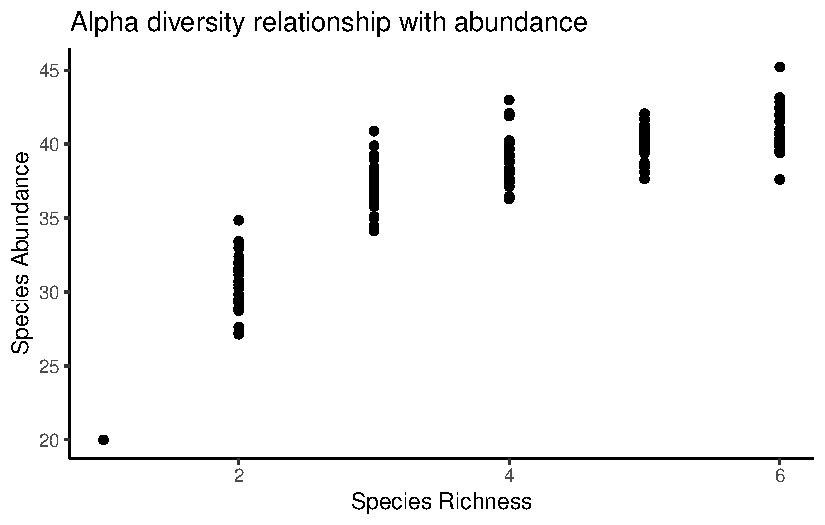
\includegraphics{Report04.04.2024_files/figure-pdf/alpha plot-1.pdf}

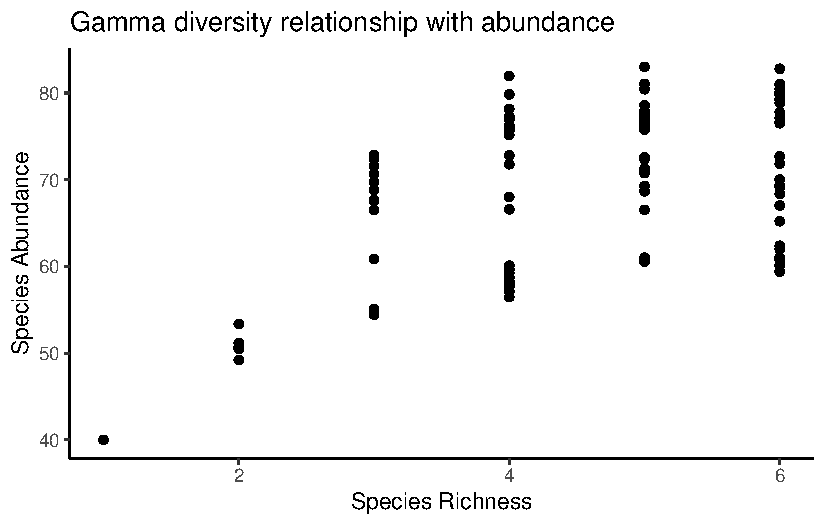
\includegraphics{Report04.04.2024_files/figure-pdf/gamma plot-1.pdf}

Okay, so I've shown that the communities and meta-communities follow a
saturated plot. The next question is when the meta-communities reach
equilibrium. In order to test this, I did a simulation over a 90 day
breeding season (Time = 90). Then, for each meta-community at each time
period I established \(\Delta\)P, or the change in abundance of each
species in each patch. I then recorded whether the \(\sum \Delta\)P was
below a critical threshold (I chose 0.01 somewhat arbitrarily). If
\(\sum \Delta\)P was below that threshold, that indicated that the
meta-community had reached equilibrium. I provide the code below for you
to review as well as a table of the first 6 meta-communities showing
when they reached equilibrium.

\begin{Shaded}
\begin{Highlighting}[]
\NormalTok{Time }\OtherTok{\textless{}{-}} \DecValTok{90} \CommentTok{\#assume a 90 day breeding season}
\NormalTok{phi }\OtherTok{\textless{}{-}} \FunctionTok{runif}\NormalTok{(}\DecValTok{6}\NormalTok{)}\CommentTok{\# Need to establish dispersal metric. May need to determine more realistic values (see notes}
\CommentTok{\# from meeting with mark + brittany on 03/28/25)}
\NormalTok{meta\_comm\_change }\OtherTok{\textless{}{-}} \FunctionTok{data.frame}\NormalTok{(}\AttributeTok{meta\_com =} \DecValTok{1}\SpecialCharTok{:}\FunctionTok{length}\NormalTok{(meta\_comm\_list), }\AttributeTok{time =} \ConstantTok{NA}\NormalTok{)}
\ControlFlowTok{for}\NormalTok{(c }\ControlFlowTok{in} \DecValTok{1}\SpecialCharTok{:}\FunctionTok{nrow}\NormalTok{(meta\_comm\_change))\{}
\NormalTok{  meta\_comm }\OtherTok{\textless{}{-}}\NormalTok{ meta\_comm\_list[[c]]}
\NormalTok{  meta\_comm\_df }\OtherTok{\textless{}{-}} \FunctionTok{data.frame}\NormalTok{(}\FunctionTok{matrix}\NormalTok{(}\FunctionTok{unlist}\NormalTok{(meta\_comm), }\AttributeTok{nrow =}\NormalTok{ num\_patches, }\AttributeTok{ncol =}\NormalTok{ num\_spp, }\AttributeTok{byrow =}\NormalTok{ T))}
  \ControlFlowTok{for}\NormalTok{(t }\ControlFlowTok{in} \DecValTok{1}\SpecialCharTok{:}\NormalTok{Time) \{}
\NormalTok{    deltaP }\OtherTok{\textless{}{-}} \FunctionTok{data.frame}\NormalTok{(}\FunctionTok{matrix}\NormalTok{(}\AttributeTok{data =} \ConstantTok{NA}\NormalTok{, }\AttributeTok{nrow =}\NormalTok{ num\_patches, }\AttributeTok{ncol =}\NormalTok{ num\_spp))}
    \ControlFlowTok{for}\NormalTok{ (i }\ControlFlowTok{in} \DecValTok{1}\SpecialCharTok{:}\NormalTok{num\_patches) \{}
      \ControlFlowTok{for}\NormalTok{(j }\ControlFlowTok{in} \DecValTok{1}\SpecialCharTok{:}\NormalTok{num\_spp) \{}
\NormalTok{        other\_patch }\OtherTok{\textless{}{-}} \FunctionTok{as.numeric}\NormalTok{(meta\_comm\_df[}\SpecialCharTok{{-}}\NormalTok{i,])}
\NormalTok{        deltaP[i,j] }\OtherTok{\textless{}{-}}\NormalTok{ phi[[j]]}\SpecialCharTok{*}\NormalTok{other\_patch[[j]] }\SpecialCharTok{{-}}\NormalTok{ phi[[j]]}\SpecialCharTok{*}\NormalTok{meta\_comm\_df[i,j]}
\NormalTok{      \}}
\NormalTok{    \}}
\NormalTok{    meta\_comm\_change[c,}\DecValTok{2}\NormalTok{] }\OtherTok{\textless{}{-}} \ControlFlowTok{if}\NormalTok{(}\FunctionTok{sum}\NormalTok{(}\FunctionTok{abs}\NormalTok{(deltaP)) }\SpecialCharTok{\textgreater{}} \FloatTok{0.01}\NormalTok{)\{ }
      \CommentTok{\#if deltaP is \textgreater{} 0 then the system is not yet at equil.}
\NormalTok{      t\} }\ControlFlowTok{else}\NormalTok{\{}
        \ControlFlowTok{next}\NormalTok{\}}
\NormalTok{    new\_abund }\OtherTok{\textless{}{-}}\NormalTok{ meta\_comm\_df }\SpecialCharTok{+}\NormalTok{ deltaP}
\NormalTok{    meta\_comm\_df }\OtherTok{\textless{}{-}}\NormalTok{ new\_abund}
\NormalTok{  \}}
\NormalTok{\}}
\FunctionTok{gt}\NormalTok{(}\FunctionTok{head}\NormalTok{(meta\_comm\_change))}
\end{Highlighting}
\end{Shaded}

\begingroup
\fontsize{12.0pt}{14.4pt}\selectfont
\begin{longtable*}{rr}
\toprule
meta\_com & time \\ 
\midrule\addlinespace[2.5pt]
1 & 56 \\ 
2 & 49 \\ 
3 & 47 \\ 
4 & 21 \\ 
5 & 46 \\ 
6 & 59 \\ 
\bottomrule
\end{longtable*}
\endgroup

I then went a step further. As an example. I plotted the simulation of
the first metacommunity over time, so visualize when it reaches
equilibrium. According to our table, you see that it should reach
equilibrium around t = 56.

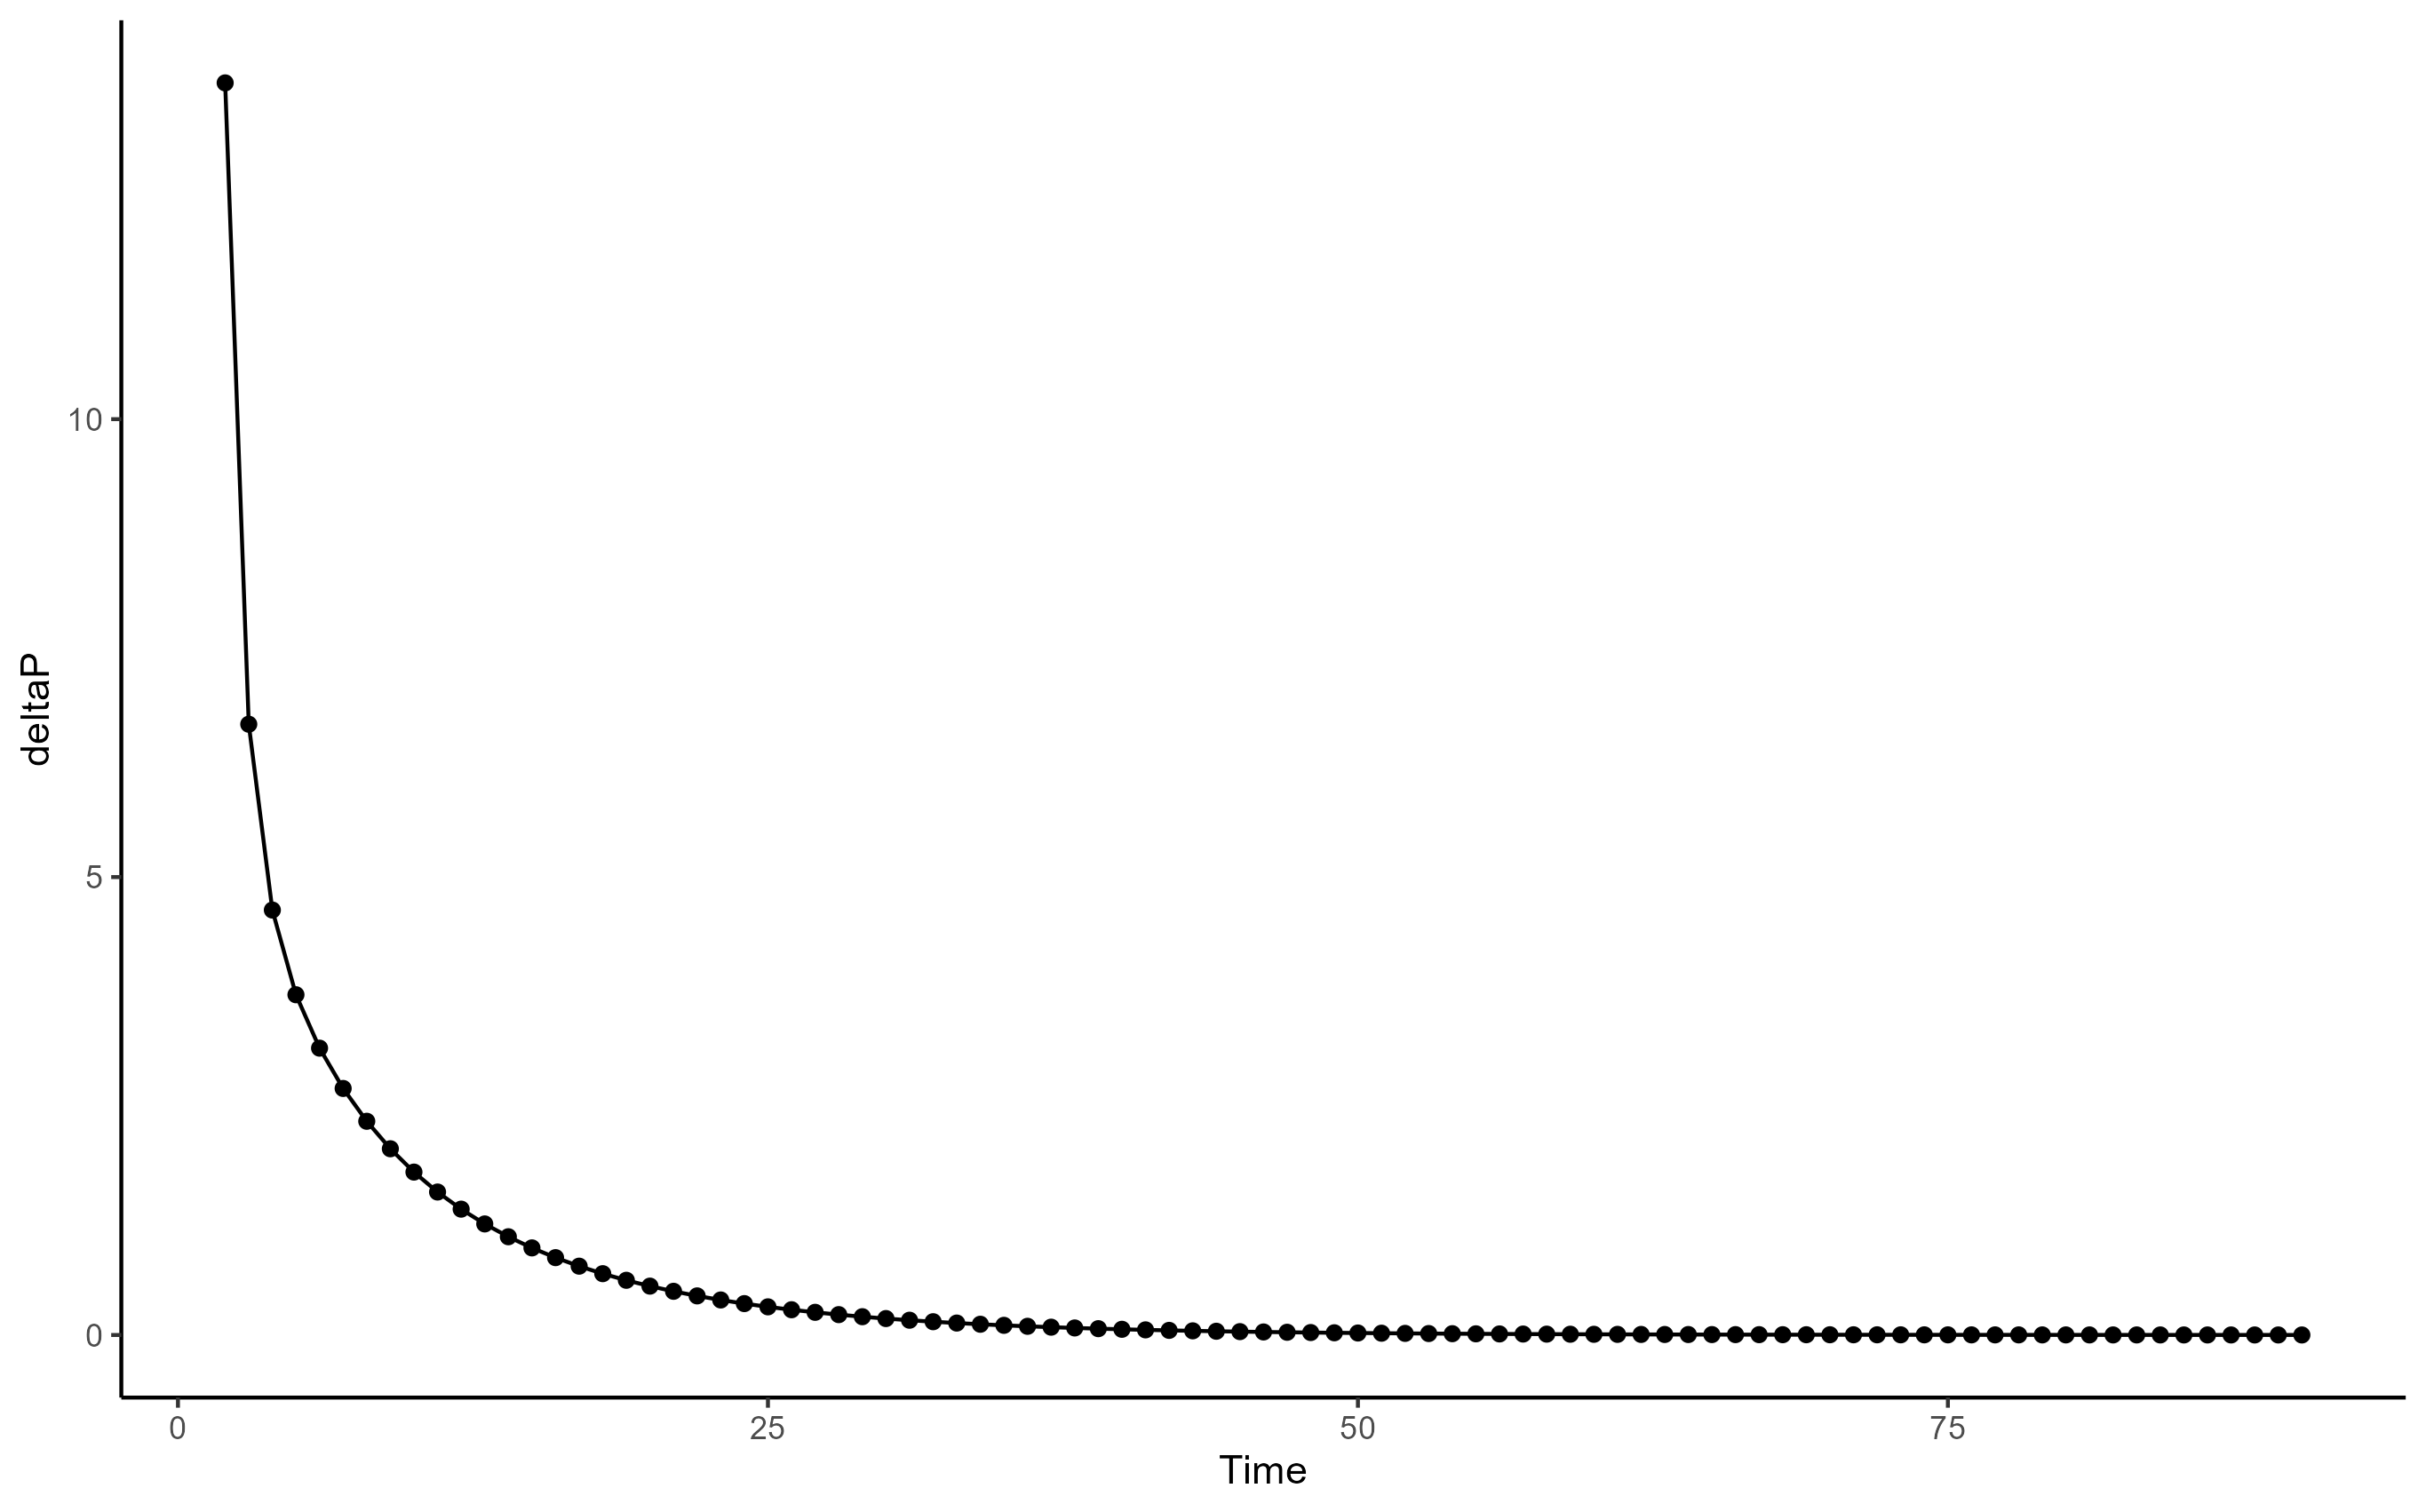
\includegraphics[width=9.1in,height=\textheight]{deltaP_plot.png}

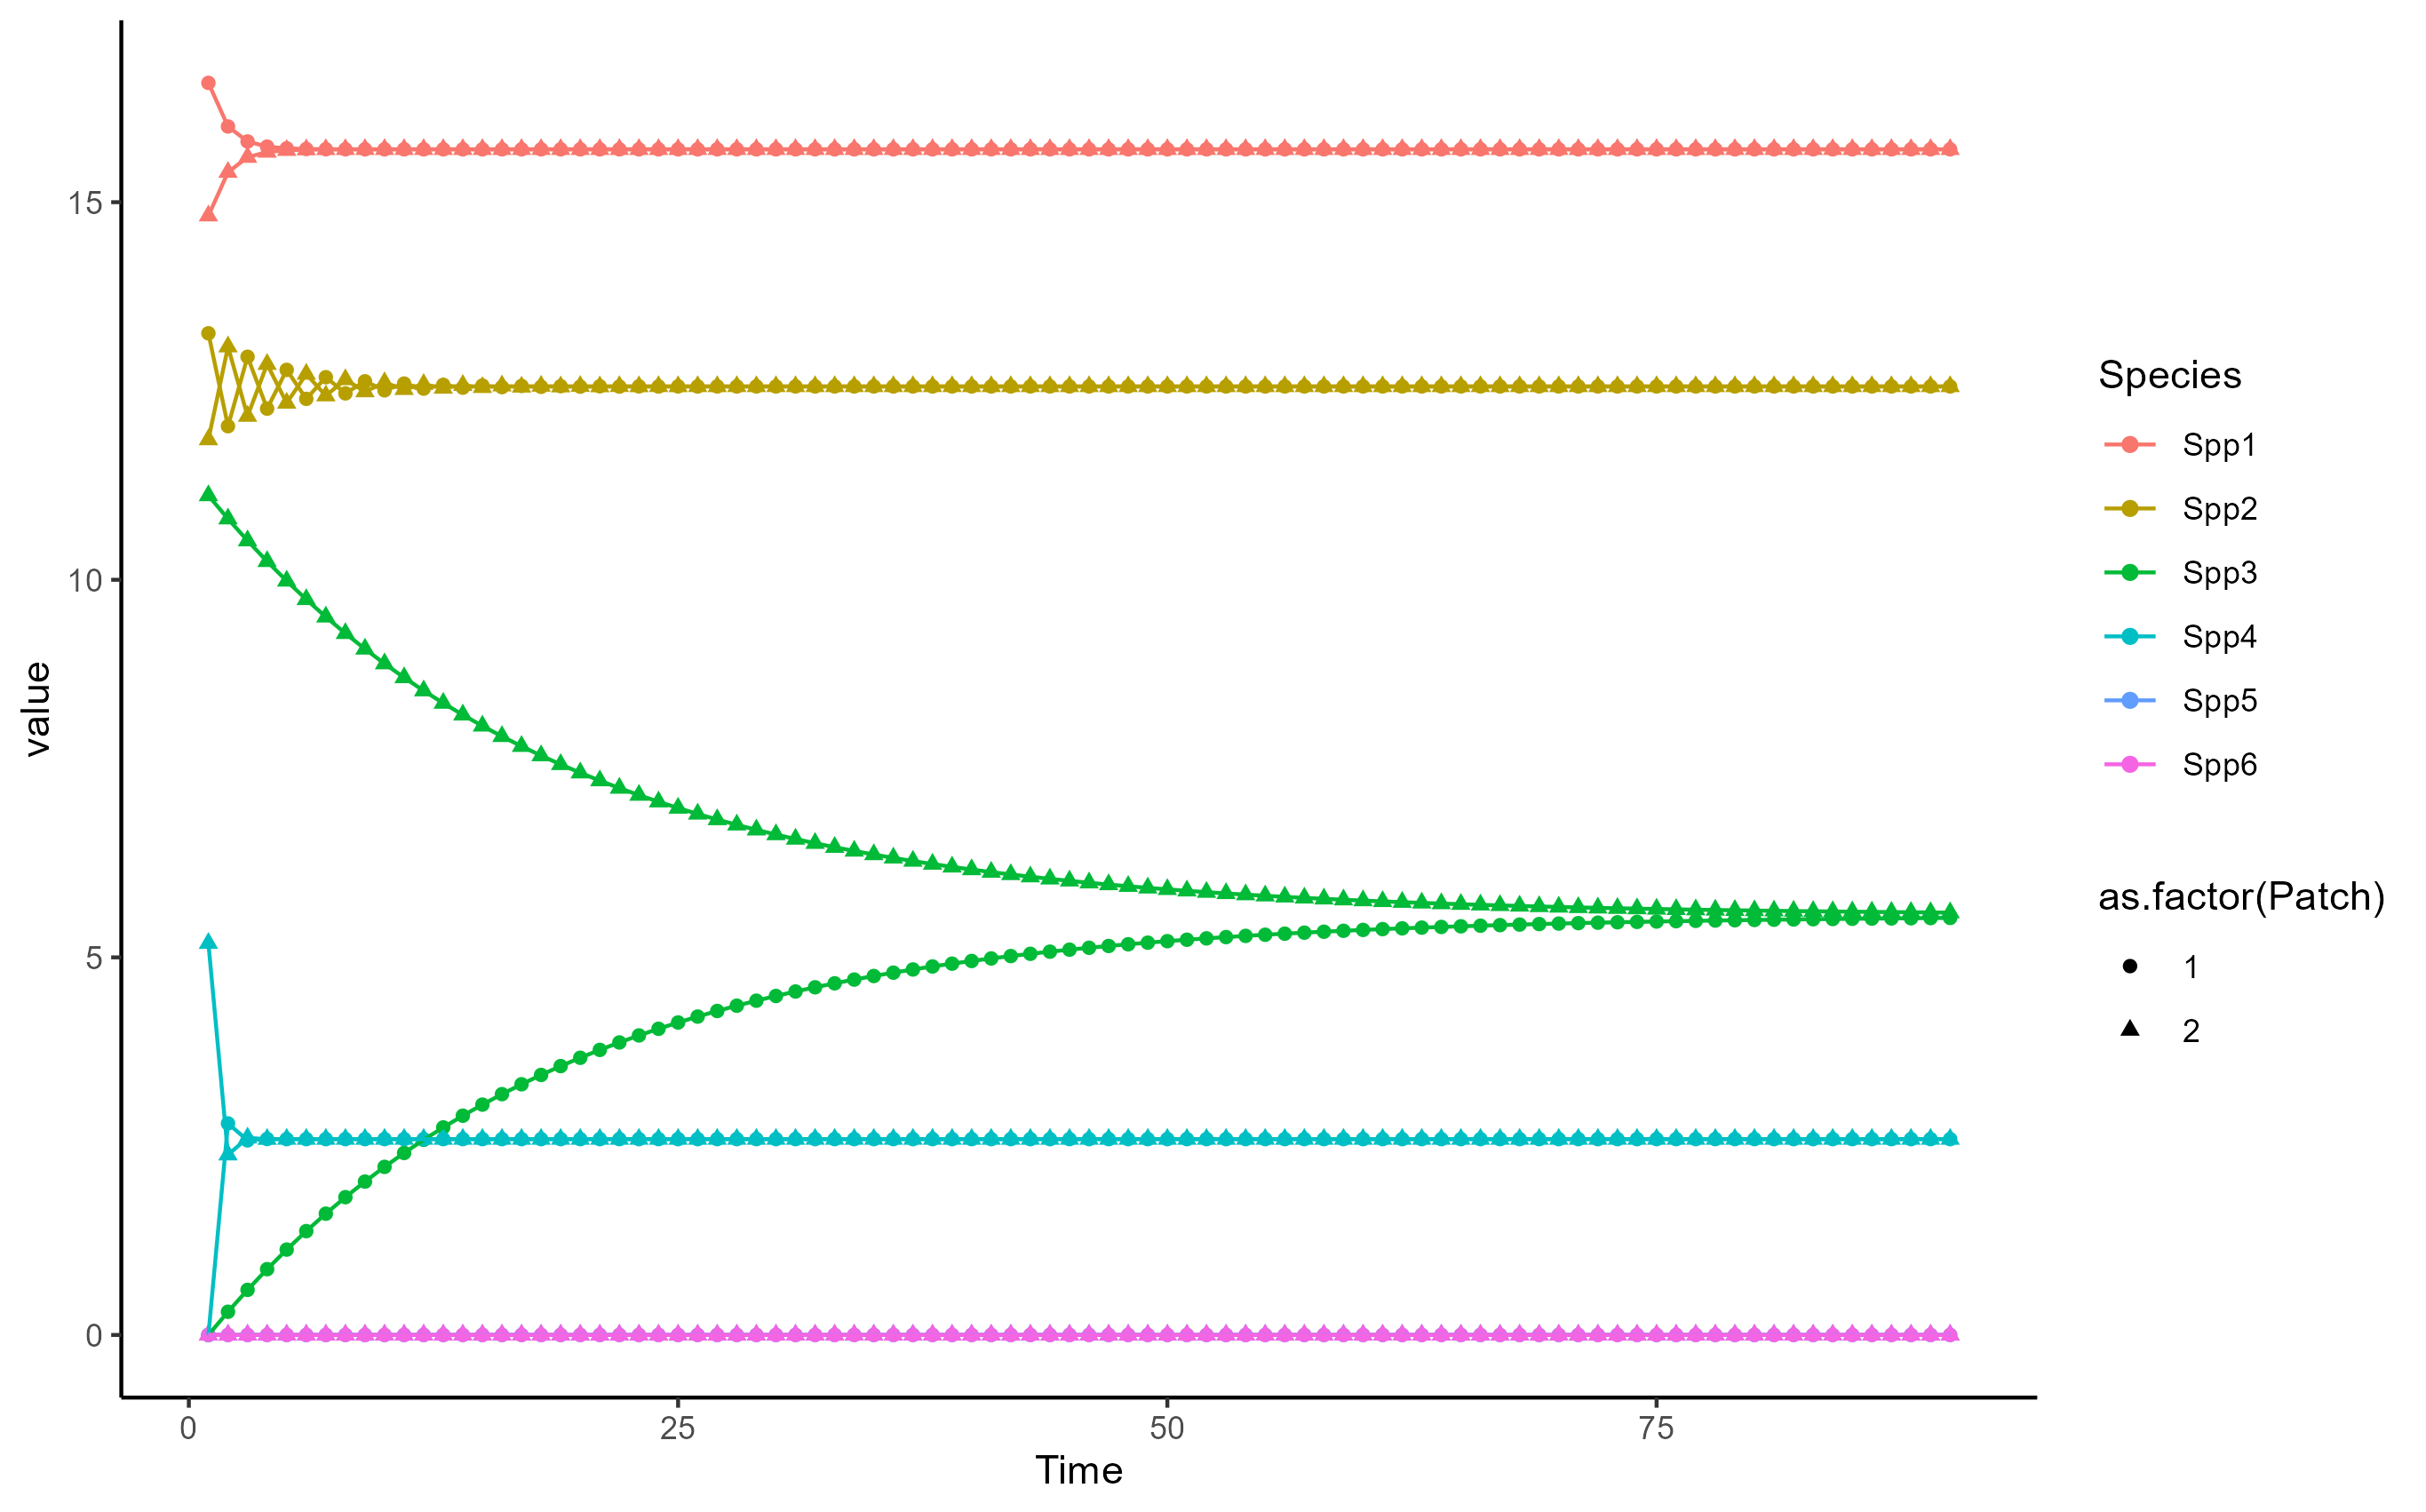
\includegraphics[width=9.1in,height=\textheight]{equil_plot.png}

So, if you look at the first plot, you see that we are in fact able to
reach an equilibrium! the change in abundance for each species becomes
effectively 0. However, there is an issue I would like to point out. The
second graph shows that as meta-communities approach equilibrium the
populations become homogenous. this could be an issue, as a key goal of
this project is to understand how the \textbf{difference} in communities
effects \(R_{0L}\) . I have some thoughts on this. My first thought is
that we could use this as an opportunity. If we were to do a time
simulation and measure \(R_{0L}\) at each time step we could show how
homogenizing the community effects disease risk in addition to assessing
the importance of \(\beta\) diversity. We could even measure \(\beta\)
at each step! This is the route that I'm leaning toward. However, we
could also play with the connectivity of patches to see if creating
heterogeneous connectivity results in a equilibrium state where patches
still differ in abundance.

These are my thoughts for the moment. Super excited at this progress and
would love to hear your thoughts!

-Reed

\phantomsection\label{refs}
\begin{CSLReferences}{1}{0}
\bibitem[\citeproctext]{ref-mihaljevic2014}
Mihaljevic, Joseph R., Maxwell B. Joseph, Sarah A. Orlofske, and Sara H.
Paull. 2014. {``The Scaling of Host Density with Richness Affects the
Direction, Shape, and Detectability of Diversity-Disease
Relationships.''} Edited by Delmiro Fernandez-Reyes. \emph{PLoS ONE} 9
(5): e97812. \url{https://doi.org/10.1371/journal.pone.0097812}.

\end{CSLReferences}




\end{document}
